\documentclass[11pt]{article}
\usepackage[margin=1in]{geometry}
\usepackage{amsmath,amssymb,booktabs,graphicx,hyperref,xcolor}
\DeclareSymbolFont{largesymbols}{OMX}{lmex}{m}{n}
\setlength{\emergencystretch}{1em}
\setcounter{topnumber}{3}
\setcounter{totalnumber}{5}
\renewcommand{\topfraction}{.9}
\renewcommand{\textfraction}{.07}
\hypersetup{colorlinks=true,linkcolor=blue,urlcolor=blue,citecolor=blue}
\newcommand{\pending}[1]{\par\noindent\textcolor{red}{[Revision evidence pending: #1]}\par}
\title{Restoring Operational Histories with Generated Temporal Graph Supervision}
\author{Author details pending final review}
\date{Working revision---not the final review manuscript}
\begin{document}
\maketitle

\begin{abstract}
An analyst investigating a purchase order or loan application needs its complete history, including cancellations and retries. Missing object links, wrong joins and fragmented identifiers can hide relevant records or introduce false evidence. We study offline repair of these associations while preserving recorded event content. Executable workflows provide training references; separate observation and fault models vary the conditions under which a learner must recover them. We evaluate the resulting supervision against models trained on the same limited number of verified operational histories, counting both fitting and calibration labels. A separate comparison adapts the author-provided HERE Transformer, without expert rules, to its supported missing-case-identifier task. Evaluation measures retrieved histories, operational queries, false identity merges and newly damaged records. The study distinguishes generated references, controlled faults in public business logs, and naturally verified corrections.
\pending{The final quantitative finding and its scope will be written only after all declared confirmation experiments finish.}
\end{abstract}

\section{Application and contribution}
A cancellation can be correctly recorded yet absent from the history retrieved for an order. A wrong join can make another customer's record appear in that history. When two systems assign different identifiers to the same object, either identifier may retrieve only part of its evidence. These failures make operational investigation difficult even when activities and timestamps themselves are accurate.

The practical objective is to restore recorded evidence, including exceptional behavior. We retain cancellations, returns and repeated work rather than changing the record to resemble an ideal process. The input is an available window of event--object relations, and the output is an auditable set of association and identity edits. This is offline reconstruction; later observations inside the window can support an earlier association.

Training such a repair system requires examples of correct histories and the ways their observed connections can fail. Verification is costly because an investigator may need to reconcile several records and identifiers. Executable workflows offer exact symbolic references, but simulated observations can contain misleading regularities. For example, an amount may be constant throughout a simulated order while the corresponding operational measurement changes between activities. A learner can mistake such differences for incorrect joins.

We therefore ask two linked application questions. Does varying observations of an unchanged workflow execution improve generated repair supervision? When some histories can be verified, does this supervision add value beyond a model using the same verification budget? The second question includes the labels needed to choose operating thresholds. Improved average retrieval is insufficient if a method introduces damaging false associations.

The contribution is an executable training-data protocol and its evaluation for coupled temporal association and identity repair. The classifiers, observation-randomization principle and graph operators are established components. The evidence includes a paired observation study, explicitly accounted adaptation budgets, a published-code comparison on a compatible task, and measurements of useful recovery and harm. The generator is a bounded component; building a universal scientific dataset platform is outside this paper.

\section{Related work and comparison scope}
HERE combines a Transformer with optional expert knowledge for missing case identifiers~\cite{here}. We retain its author model, tensor dataset and greedy decoder in a separate single-case comparison. Its output contract does not directly express simultaneous multi-object participation edits and alias merging. SANAGRAPH repairs event-log attributes using supplied trace structure~\cite{sanagraph}; providing correct trace membership would expose a target of our task. DDTR and process-tree approaches recover trace content~\cite{ddtr,processtree}. Their objectives differ from preserving event content while restoring its associations.

Contextual Event Knowledge Graph inference uses available relations and physical rules to infer missing entity identifiers~\cite{ekginference}. Object-centric imperfection patterns identify association and identity problems encountered in practice~\cite{ocip}. Their public artifacts include injected event--object faults and observed cross-log object--object disagreements. The latter are useful evidence of data inconsistency, but do not independently certify the missing or wrong event--object links evaluated here. We do not claim to introduce these error categories.

Object-centric simulation~\cite{ocsim}, configurable process-data faults~\cite{flawd}, and temporal graph generation~\cite{tigger} supply relevant building blocks. Domain randomization is an established transfer strategy~\cite{domainrandomization}; synthetic relational pretraining also has recent precedents~\cite{plurel,rdbpfn}. Our question concerns what these ideas buy an operational repair application under explicit information and verification limits. HoloClean illustrates joint evidence-based data repair~\cite{holoclean}; the present study concentrates on temporal histories, their identity fragmentation and the consequences of repairing them.

\section{Task and executable supervision}
\subsection{Observed information and permitted edits}
An event is $e=(u,t,a,P,x)$: an opaque handle, time, activity, typed participants and legitimate descriptive fields. Event--object incidence and temporal adjacency within observed histories form the temporal graph. Equal-time records remain simultaneous; source row order supplies no causal ordering. A typed catalog contains the available object handles, including any aliases.

The system can add or remove participation and merge same-type aliases. It cannot invent events, change recorded activities or times, create entirely unknown entities, or split an already overmerged identity. A merge consolidates handles and deduplicates participation. These capabilities matter when choosing a dataset: natural errors requiring a different operation cannot validate this repair vocabulary.

Only the observed graph and target-type schema enter inference. The canonical identity map, clean case containers, corruption locations, seeds and clean-derived adjacency remain outside the learner interface. Target links are corrupted while resources and, where available, vendors remain context. This is a scoped fault model, not evidence of robustness to unreliable timestamps or pervasive context corruption. Public logs provide reference representations for controlled fault injection; they are not certifications that every underlying business record is correct.

\subsection{Generate execution, observation and recording faults separately}
Executable worlds contain parents, work items, resources and optional batches. Mechanisms include branching, joins, resource queues, handoffs, multistage routes, repeated work, cancellations and returns. Queueing configurations enforce resource capacity. The worlds are symbolic workflows, not calibrated digital twins of the evaluated organizations.

Observation projection determines visible entity types and fields. Recording faults are applied afterwards, producing learner observations and separate participation/identity references. Normalized recipes, random states, source fingerprints and export hashes record provenance. Execution checkpoints reproduce uninterrupted runs. Observations sharing an execution stay in the same data split.

The paired observation comparison holds executed events, timestamps, target types and faults fixed. Generated views retain original fields or introduce activity-dependent categories, noisy numerical measurements, incidental categories and time bands, with varying field availability. Measurements can depend on an observed amount and activity, but never on a target identifier. Clean and damaged versions receive aligned descriptions through builder-only execution ancestry. Each trial contains 512 fitting worlds and 96 generated calibration worlds. Three independently generated collections test sensitivity to generated training data.

The mixed fault family splits eligible histories at a temporal cut with probability .25, removes approximately .10 of each resulting handle's links in a contiguous block, and replaces surviving target links with probability .10 by a different same-type identity. Histories require at least four events to be fragmented. Missing-block widths use stochastic rounding so short histories can also lose links. A separately implemented pipeline stressor uses activity-routed aliases, a recording outage and persistent stale joins. These are declared experimental conditions, not estimates of natural incident rates.

\begin{figure}[t]
\centering
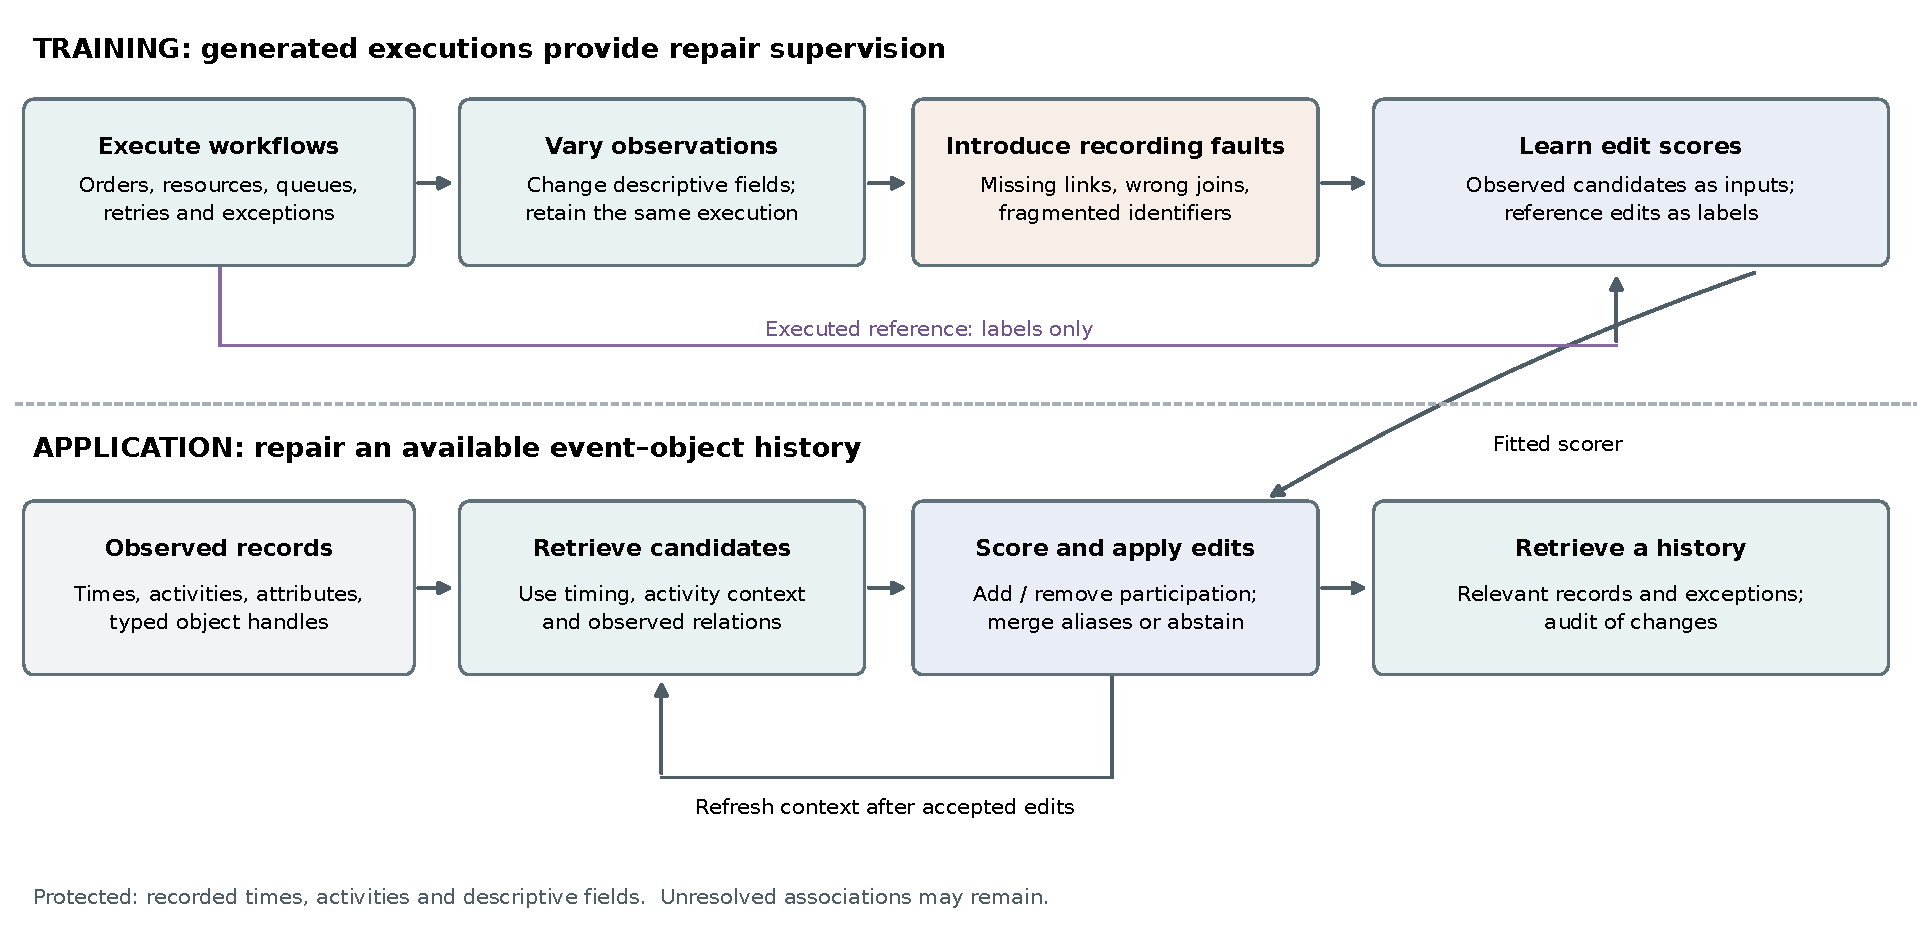
\includegraphics[width=\linewidth]{../../paper/figures/method_overview.pdf}
\caption{Executable references supervise repair training. Inference uses the observed temporal graph and preserves recorded event content. Reference identities and fault locations remain outside learner input.}
\label{fig:method}
\end{figure}

\subsection{Learn and apply auditable edits}
Candidate retrieval uses temporal proximity, activity, co-participation and descriptive agreement. Participation features summarize history degree, temporal bracketing, transitions and contextual agreement. The query event is excluded from the evidence supporting its existing association. Identity features compare temporal boundaries and activity, context and field profiles. Opaque identifier values are not numerical predictors.

Separate boosted classifiers score additions, removals and merges. An addition is labelled correct when it supplies a missing reference entity; a removal when the current entity is incorrect; a merge when both handles refer to the same entity. Generated training includes partial teacher-repaired states. These local targets do not guarantee improvement in final history retrieval. Earlier neural controls use the same candidates with MLP, GraphSAGE~\cite{graphsage} or temporal message-passing scorers; architecture superiority is not our contribution.

The decoder selects a commuting batch, applies it, recomputes observed evidence and repeats for at most four passes in the revision experiments. It cannot simultaneously merge an entity and edit its participation. Accepted participation edits are not reversed; accepted merges cannot be split by inference. Every batch retains a reversible audit record. For operational graphs, candidate limits are 128 participants per event/type and 64 identity candidates per anchor. Candidate coverage is reported separately from scoring accuracy.

\section{Verified-history budgets and evaluation}
\subsection{Public sources and prospectively assigned cohorts}
Loan data come from BPI 2017~\cite{bpi2017}. Targets are applications and explicitly referenced offers; resources are context. Purchasing data use the released BPI 2019 OCEL representation~\cite{bpi2019,bpiconversion,bpiocel}; targets are purchase orders and items, with resources and vendors as context. Identifiers and copied trace/object fields are removed from learner attributes. The loan adapter retains allowed event-level descriptions; the purchasing adapter retains cumulative net worth. An absent native offer link is not treated as proof that no real-world relationship existed.

The revision excludes the earlier feasibility prefixes, earlier confirmation roots and their target children. Roots sharing target children, or crossing an excluded target child, are also excluded. A declared hash ranking assigns 512 development, 1,024 annotation and 1,024 confirmation roots per source, followed by a separate native-method block. Associated target children stay with their root; context resources and vendors may overlap. The native block was prospectively extended from 256 to 2,048 roots for a credible training volume, before its outcomes were inspected. All preceding root partitions were checked to remain unchanged.

The main confirmation cohorts contain 39,421 loan events and 21,680 purchasing events. The native-method cohorts contain 77,981 and 40,483 events. These are fresh object histories from previously studied processes, not new institutions or untouched source domains. Earlier study outcomes inform revision development and are identified separately from the new confirmation.

\subsection{Count fitting and calibration together}
A verification unit is a complete root history bundle: the root, its target children, all their alias handles and their event memberships. A restricted label view exposes exactly the selected bundles. It cannot reveal the canonical identities of unselected histories. Complete alias verification makes an unlisted candidate a valid negative for a selected entity; this assumption must hold for the simulated verification protocol to represent real annotation.

Total budgets of 16, 64 and 256 bundles allocate 12/48/192 to fitting and 4/16/64 to calibration. Hash-based assignments are nested, and a root retains its role as the budget increases. Three allocation/fault seeds are retained. Table~\ref{tab:annotation-cost} counts verified events, entities and aliases; the artifact also records sampled queries. Each role uses at most 4,096 event queries; the complete verification cost is still counted. These are simulated reference accesses, not measured human work hours.
\begin{table}[t]
\centering
\begin{tabular}{llrrr}
\toprule
Source & Bundles & Verified events & Target entities & Alias handles \\
\midrule
Loans & 16 & 586--672 & 36--44 & 41--54 \\
Loans & 64 & 2,317--2,388 & 152--159 & 178--185 \\
Loans & 256 & 9,132--9,533 & 600--614 & 703--740 \\
Purchasing & 16 & 204--880 & 51--178 & 63--218 \\
Purchasing & 64 & 1,333--1,844 & 275--398 & 337--478 \\
Purchasing & 256 & 5,448--5,947 & 1,170--1,434 & 1,438--1,725 \\
\bottomrule
\end{tabular}
\caption{Total simulated verification access, including fitting and calibration. Ranges cover the three declared allocation/fault seeds. A complete bundle includes associated target children and all their aliases. Counts are not measured annotator time; query subsampling does not reduce the reported verification cost.}
\label{tab:annotation-cost}
\end{table}


Real-only, original-generated-plus-real and varied-generated-plus-real classifiers receive identical real labels at each budget. Hyperparameters are fixed: 200 boosting iterations, 15 leaves, learning rate .08, regularization 1 and no early stopping. Mixed fitting initially gives generated and real examples equal weight mass, followed by class balancing. The generated collection is held fixed across these adaptation seeds. If fitting lacks a positive or negative class for an operation, that operation abstains.

Calibration chooses the highest-recall threshold attaining empirical precision of at least .95 and at least five correct actions for each operation. An infeasible operation abstains. A zero-budget control uses generated calibration. A calibration-only control spends the complete selected target budget on thresholds for fixed generated weights, without target fitting. It uses the same selected bundles as the fitting-plus-calibration comparisons. Thus calibration is neither free nor silently supplied from another labelled target set. Historical research and development labels are additional costs; these curves measure incremental adaptation to new histories in known processes.

\subsection{Measure useful recovery and introduced errors}
For reference entity $q$, let $H_q$ be its event history, $A_q$ its observed aliases, and $\widehat H(u)$ the events retrieved by the predicted cluster of handle $u$. The primary outcome is
\[
 F_{\mathrm{history}}=\frac{1}{|Q|}\sum_{q\in Q}\frac{1}{|A_q|}
 \sum_{u\in A_q}\frac{2|\widehat H(u)\cap H_q|}{|\widehat H(u)|+|H_q|}.
\]
Entities with no reference events do not enter $Q$. Exact-history recovery replaces the inner score by an equality indicator, retaining the same entity/alias weighting. It does not require every alias of an entity to succeed simultaneously.

We separately measure identity-pair precision/recall and changes to initially correct events. The revised damage measure expands each predicted cluster to \emph{all} its reference identities before checking participation. Consequently, a false merge can damage events on both sides, including events whose representative handle did not change. Direct assignment damage is also retained for comparison with the earlier study. Event activity, timestamp and fields are checked to remain unchanged.

Application queries ask whether a retrieved history contains recorded cancellation evidence and whether its first/last timestamps are recovered. Cancellation evidence uses the case-insensitive substring \texttt{cancel} consistently in predictions and references. It does not establish the final business outcome, and boundary timestamps do not certify every simultaneous boundary record. Three-seed means and observed ranges summarize the declared trials; events are not treated as independent statistical replications.

\subsection{Reliability and published-method controls}
The reliability study tests a simple schema control where the public representation declares exactly one root per event. Removing a sole root requires a supported replacement, committed in the same batch. A missing root can receive one supported candidate. Other target types and alias decisions retain the original decoder rules. The middle 64-bundle budget and real-only/varied-mixture regimes are fixed for development comparison. A stricter .99 empirical-precision operating point for the original decoder is essential: a more complex control is useful only if it improves recovery at comparable damage. This control imposes an explicit application schema and does not guarantee correct identities.

The native comparison independently masks each event's single root identifier with probability .30 in each 2,048-root cohort, using three fixed seeds. Activity, resource and time are available; child identifiers, vendor relations and descriptive fields are removed for every method. Trusted remaining case IDs provide closed-case supervision. HERE's author Transformer uses 512-dimensional states, three layers, eight heads, 15-event windows, batch size eight and 30 epochs. The final epoch is evaluated. Only retained identifiers enter training targets; overlapping-window validation is diagnostic, not an independent test. The headless runner and masking/evaluation protocol are explicit adaptations. No expert rules are supplied, so the comparison is named \emph{HERE-Transformer without expert rules}, not a reproduction of the complete published system.

Matched controls include both fixed generated scorers, a target-local boosted scorer and nearest-known-event matching. Generated scorers choose one candidate for each missing ID. The local boosted control fits at most 4,096 retained-ID queries with leave-query-out profiles, whereas HERE uses the remaining known events throughout its training windows; this unequal fitting volume is reported. All retained memberships are observed context. Existing IDs remain unchanged. Native results therefore assess missing-ID completion, not robustness to wrong existing IDs, coupled alias repair or verification-budget efficiency. Data, weights, code and all six native jobs were pinned before native outcomes.

\section{Results and application interpretation}
\IfFileExists{results.tex}{\subsection{Untouched-history confirmation}
\label{sec:fresh}
\begin{table}[t]
\centering\small
\setlength{\tabcolsep}{4pt}
\caption{Untouched-history confirmation: means over eight disjoint 128-root blocks and three fixed fitted-model/fault seeds. $R_8$ repeatedly corrupts the same verified histories; $+G$ adds generated training. Budgets include calibration. $R$ counts fully recovered events and $H$ newly damaged events per block; all false-merge effects are included. History F1 is percent.}
\label{tab:fresh-primary}
\begin{tabular}{lrr rr rr rr}
\toprule
Source & Budget & $q$ & F1 $R_8$ & F1 $+G$ & $R$ $R_8$ & $R$ $+G$ & $H$ $R_8$ & $H$ $+G$ \\ \midrule
Loans & 16 & 0.95 & 80.0 & 80.0 & 65.8 & 58.5 & 6.38 & 2.21 \\
 & 16 & 0.99 & 79.8 & 79.9 & 55.6 & 32.4 & 3.71 & 0.42 \\
 & 64 & 0.95 & 82.0 & 80.2 & 226.6 & 98.2 & 2.96 & 1.25 \\
 & 64 & 0.99 & 79.9 & 79.6 & 30.2 & 62.5 & 2.08 & 0.00 \\
 & 256 & 0.95 & 81.1 & 80.7 & 110.4 & 94.1 & 1.38 & 1.71 \\
 & 256 & 0.99 & 80.1 & 80.0 & 42.2 & 34.2 & 0.75 & 3.58 \\
\midrule
Purchasing & 16 & 0.95 & 82.8 & 80.8 & 390.0 & 273.4 & 16.54 & 15.00 \\
 & 16 & 0.99 & 80.5 & 80.7 & 271.0 & 255.8 & 7.88 & 12.21 \\
 & 64 & 0.95 & 83.5 & 82.3 & 565.2 & 455.4 & 15.79 & 26.62 \\
 & 64 & 0.99 & 81.0 & 80.3 & 400.3 & 329.2 & 5.42 & 16.62 \\
 & 256 & 0.95 & 81.3 & 80.4 & 414.7 & 369.3 & 6.42 & 6.92 \\
 & 256 & 0.99 & 79.6 & 77.9 & 309.3 & 207.5 & 1.25 & 1.33 \\
\bottomrule
\end{tabular}
\end{table}

The prespecified loan result replicates (Table~\ref{tab:fresh-primary}). At 64 verified bundles and $q=.99$, augmentation raises mean full-event recovery from 30.2 to 62.5 per block and reduces new damage from 2.08 to 0.00. After averaging the three fixed model/fault runs within each block, recovery improves in all eight blocks. Fitted-seed sensitivity remains: the three seed-specific recovery differences, averaged across blocks, are 5.5, -11.5 and 103.0 events. Thus one fitted-seed mean loses recovery; block uncertainty does not cover new training draws. The paired recovery difference is 32.3 events [95\% interval 29.5, 35.3], and the damage difference is -2.08 [-3.75, -0.75]. H1 meets both its directional and interval criteria. However, history F1 decreases by 0.23 percentage points: its paired difference is -0.23 [-0.30, -0.18]. The confirmed benefit concerns recovery and harm at this operating point, not uniform improvement in every endpoint.

Table~\ref{tab:fresh-primary} also retains the failures. At 256 bundles, augmentation lowers mean history F1 and recovery and increases mean damage in both sources at both targets; not every damage interval excludes zero. On purchasing at 64 bundles it reduces recovery and increases damage at both targets. Its small purchasing F1 gain at 16 bundles and $q=.99$ accompanies fewer full-event recoveries and more damage. Thus generated data can add value beyond repeated corruption, but the evidence supports a narrow operating condition rather than a general verification-budget saving or a universal rule for when to stop generating data.

The never-merge control changes the safety interpretation (Tables~\ref{tab:fresh-safety} and~\ref{tab:fresh-contrasts}). For real-only loans, guarding reduces damage from 38.12 to 2.08, while recovery changes from 30.17 to 30.21. Never merging further reduces damage to 0.29 with the same 30.2 recoveries, but gives up 2.75 true merged pairs and some history F1. On purchasing, guarded real-only/augmented policies retain 9.46/16.08 true pairs per block. Their history F1 exceeds never merge, but their damage is 5.42/16.62, versus 4.71/15.38. The corresponding extra-harm intervals are positive. None of the four H2 comparisons establishes a beneficial merge policy without added harm over never merge.

The strict augmented loan model makes no merges under any of the three policies; all three produce identical outcomes. Its zero observed harm therefore does not demonstrate an incremental guard benefit. Moreover, real-only never merge still recovers 30.2 events versus 62.5 for the augmented model, so the recovery advantage is not explained solely by false merges in the real-only comparator. Never merging eliminates false identity merges by construction, but participation repairs can still damage records. The choice between retaining fragmented histories and accepting residual merge risk remains an application decision; the measured frontier supplies evidence, not a deployment safety guarantee.

All 768 saved repair programs passed independent replay, exact undo, event-content preservation and recomputed history/identity and cluster-expanded damage checks. The source-selection audit verified all older partition hashes and complete coverage of the declared new roots. No new fitting or threshold search was performed. Complete per-block/per-seed outcomes, conditional intervals and measured evaluation costs accompany the manuscript.

\begin{table}[t]
\centering\small
\setlength{\tabcolsep}{4pt}
\caption{Merge-policy confirmation at 64 verified bundles and $q=.99$. $R$ and $H$ are fully recovered and newly damaged events. TP/FP count true/false merged identity pairs. Never merge retains the guarded participation rules and atomic root replacements. Counts and F1 (percent) average the same 24 runs per setting.}
\label{tab:fresh-safety}
\begin{tabular}{lll rrrrr}
\toprule
Source & Arm & Policy & F1 & $R$ & $H$ & TP & FP \\ \midrule
Loans & $R_8$ & Unguarded & 80.0 & 30.2 & 38.12 & 5.21 & 3.17 \\
 &  & Guarded & 79.9 & 30.2 & 2.08 & 2.75 & 0.38 \\
 &  & Never merge & 79.6 & 30.2 & 0.29 & 0.00 & 0.00 \\
 & $+G$ & Unguarded & 79.6 & 62.5 & 0.00 & 0.00 & 0.00 \\
 &  & Guarded & 79.6 & 62.5 & 0.00 & 0.00 & 0.00 \\
 &  & Never merge & 79.6 & 62.5 & 0.00 & 0.00 & 0.00 \\
\midrule
Purchasing & $R_8$ & Unguarded & 81.0 & 400.0 & 10.54 & 11.17 & 1.75 \\
 &  & Guarded & 81.0 & 400.3 & 5.42 & 9.46 & 0.33 \\
 &  & Never merge & 80.5 & 400.9 & 4.71 & 0.00 & 0.00 \\
 & $+G$ & Unguarded & 80.5 & 327.2 & 27.54 & 21.42 & 3.17 \\
 &  & Guarded & 80.3 & 329.2 & 16.62 & 16.08 & 0.38 \\
 &  & Never merge & 79.4 & 331.0 & 15.38 & 0.00 & 0.00 \\
\bottomrule
\end{tabular}
\end{table}


\begin{table}[t]
\centering\footnotesize
\setlength{\tabcolsep}{4pt}
\caption{Prespecified contrasts at 64 bundles and $q=.99$: mean differences [conditional 95\% intervals]. The first row tests augmentation with guarded decoding; other rows subtract never merge from guarded decoding. F1 differences are percentage points; recovery and harm are events per 128-root block. Intervals resample eight blocks after averaging three fixed model/fault runs; no multiplicity correction is applied.}
\label{tab:fresh-contrasts}
\begin{tabular}{ll rrr}
\toprule
Source & Contrast & $\Delta$ F1 & $\Delta R$ & $\Delta H$ \\ \midrule
Loans & $+G-R_8$ & -0.23 [-0.30, -0.18] & 32.3 [29.5, 35.3] & -2.08 [-3.75, -0.75] \\
Loans & $R_8$: guard--never & 0.27 [0.20, 0.35] & 0.0 [0.0, 0.0] & 1.79 [0.54, 3.38] \\
Loans & $+G$: guard--never & 0.00 [0.00, 0.00] & 0.0 [0.0, 0.0] & 0.00 [0.00, 0.00] \\
Purchasing & $R_8$: guard--never & 0.52 [0.42, 0.63] & -0.6 [-1.0, -0.2] & 0.71 [0.25, 1.17] \\
Purchasing & $+G$: guard--never & 0.85 [0.76, 0.93] & -1.8 [-2.8, -1.0] & 1.25 [0.62, 1.87] \\
\bottomrule
\end{tabular}
\end{table}


\subsection{Exploratory repeated-corruption study}
\label{sec:followup}
The precursor study fitted 60 models and evaluated 156 repair conditions, including the full-input models reused for confirmation and the input ablations below. Choices were frozen before the new model outcomes. Evaluation uses 128 hash-selected roots from each previously evaluated confirmation cohort: 4,942 loan and 2,792 purchasing events. These reused source histories make this an exploratory follow-up, not independent confirmation. A single simultaneous proposal pass commits root replacements atomically. Both fixed calibration targets, .95 and .99, are reported. A guard rejects tied additions and permits merges only at score at least .99, without co-occurring handles, and with mutual-best scores separated from alternatives by .05. The same guard applies to both training arms. Its observed harm must still be measured; score thresholds are not guarantees. Different cohort size, context and decoding make these scores non-comparable to the earlier four-pass results.

\begin{table}[t]
\centering\small
\caption{Repeated-corruption follow-up: three-seed means on 128 reused roots per source. $R_8$ uses eight corruptions of each verified fitting set; $+G$ adds generated histories. $q$ is the calibration precision target. Recovery and damage count fully corrected initially incorrect events and newly incorrect initially correct events, with alias expansion. Equal $q$ does not guarantee equal test damage.}
\label{tab:repeated-corruption}
\setlength{\tabcolsep}{4pt}
\begin{tabular}{lrr rr rr rr}
\toprule
 & & & \multicolumn{2}{c}{History F1 (\%)} & \multicolumn{2}{c}{Recovered} & \multicolumn{2}{c}{Damaged} \\
Source & Budget & $q$ & $R_8$ & $+G$ & $R_8$ & $+G$ & $R_8$ & $+G$ \\ \midrule
Loans & 16 & 0.95 & 79.2 & 79.4 & 64 & 67 & 10.0 & 4.0 \\
 & 16 & 0.99 & 78.9 & 79.2 & 55 & 35 & 6.7 & 1.3 \\
 & 64 & 0.95 & 81.6 & 79.6 & 237 & 108 & 1.7 & 1.7 \\
 & 64 & 0.99 & 79.2 & 79.0 & 30 & 67 & 0.0 & 0.0 \\
 & 256 & 0.95 & 80.5 & 80.0 & 123 & 102 & 2.3 & 2.3 \\
 & 256 & 0.99 & 79.4 & 79.2 & 46 & 38 & 1.7 & 1.0 \\
\midrule
Purchasing & 16 & 0.95 & 82.7 & 80.9 & 388 & 257 & 25.0 & 19.3 \\
 & 16 & 0.99 & 80.5 & 81.0 & 269 & 236 & 7.7 & 13.0 \\
 & 64 & 0.95 & 83.5 & 82.6 & 501 & 423 & 15.7 & 10.0 \\
 & 64 & 0.99 & 81.1 & 80.5 & 343 & 309 & 2.7 & 4.7 \\
 & 256 & 0.95 & 81.3 & 80.7 & 350 & 347 & 7.7 & 6.7 \\
 & 256 & 0.99 & 79.7 & 78.2 & 253 & 196 & 1.7 & 1.3 \\
\bottomrule
\end{tabular}
\end{table}


Table~\ref{tab:repeated-corruption} gives the complete budget/threshold comparison. A useful conditional result occurs on loans at budget 64 and $q=.99$: generation raises mean fully recovered events from 30.3 to 67.0 with zero observed new damage in either arm. It improves recovery in two seeds and loses in one; mean history F1 is slightly lower. At $q=.95$, the same augmentation reduces recovery from 236.7 to 108.3 at equal mean damage. Purchasing at budget 64 trades fewer recoveries for less damage at .95, but loses on both measures at .99. At budget 256, augmentation lowers mean history F1 in both sources at both targets. This fixed mixture therefore offers no established general advantage beyond repeated corruption; neither a universal verification-budget saving nor the optimal point to stop using generation follows from these trials.

Table~\ref{tab:followup-ablation} removes information before retrieval and refitting. On loans, removing timestamps reduces mean full-event recovery from 108.3 to 7.7, also reducing damage. Purchasing loses history F1 without context objects or descriptions. Descriptions are not uniformly beneficial: removing them slightly improves loan F1 and recovery while increasing damage. Removing all history edges yields no repairs. These results identify information dependencies of the scorer and candidate pipeline; they do not establish superiority of a graph neural architecture.

At budget 64 and .99, the guard reduces real-only loan damage from 39.7 to 0.0 events while preserving 30.3 recoveries, but reduces correctly merged identity pairs from 5.3 to 1.7. For augmented purchasing, damage falls from 10.3 to 4.7 with recovery changing from 307.7 to 308.7; some false pairs remain. All 192 empty-history model--event decisions remain unresolved both with and without the guard, so this challenge establishes no incremental guard benefit. Guarded augmented purchasing still damages 5.3 events on clean inputs and recovers only 54.0 events while damaging 39.3 under pipeline faults. Pipeline faults appear in training; this is a known-family stress test.

On a Threadripper PRO 5955WX with four fitting threads per worker, budget-64 real-only/augmented fitting takes mean 3.5/5.7 seconds for loans and 4.6/7.1 for purchasing. The shared generated feature cache costs 10.1 seconds; full-input inference including candidate construction and metric computation takes about 33/21 seconds per loan/purchasing test graph, excluding file writes. These are measured host timings, not human verification savings. All 60 calibration computations and 156 saved repairs were replayed; independent checks verified history metrics, cluster-expanded harm, event preservation and exact undo. Per-seed ranges and full costs remain in the artifact; the artifact includes the fixed recovery--damage frontier.


\begin{table}[t]
\centering\small
\caption{Input ablations of $+G$, budget 64, $q=.95$: three-seed means. Information is removed before retrieval and fitting. No-context retains target root/child incidence; no-history removes incidence from the evidence index. These are information ablations, not architecture comparisons.}
\label{tab:followup-ablation}
\begin{tabular}{l rrr rrr}
\toprule
 & \multicolumn{3}{c}{Loans} & \multicolumn{3}{c}{Purchasing} \\
Input & F1 (\%) & Recovered & Damaged & F1 (\%) & Recovered & Damaged \\ \midrule
All information & 79.6 & 108 & 1.7 & 82.6 & 423 & 10.0 \\
No timestamps & 78.4 & 8 & 0.0 & 81.7 & 424 & 7.3 \\
No context objects & 79.4 & 81 & 2.0 & 80.9 & 327 & 8.3 \\
No descriptions & 79.9 & 137 & 4.7 & 80.2 & 358 & 12.0 \\
No history edges & 78.3 & 0 & 0.0 & 76.2 & 0 & 0.0 \\
\bottomrule
\end{tabular}
\end{table}




\subsection{Earlier evidence and comparator sensitivity}
The earlier paired observation study held executions and faults fixed while varying visible generated fields. Varied supervision raised mean history F1 from .791 to .805 on loans and from .809 to .826 on purchasing; a separate 96-world generated confirmation improved from .759 to .800. Limits were also visible: the loan pipeline condition decreased F1 in all three trials, and real-source training outperformed generated transfer on the BPI 2012 check. The full paired table and failures remain in the artifact.

The earlier combined-repair experiment evaluated 156 declared conditions on 1,024-root cohorts, using one real corruption view and four decoding passes. On purchasing, the varied mixture with 64 verified bundles reached 85.6\% history F1 versus 80.6\% for real-only training, winning all three paired trials; it also exceeded the 84.5\% real-only mean at 256 bundles. It raised exact-history recovery from 36.5\% to 48.7\% and fully recovered 3,880 initially incorrect events versus 2,992, while damaging 237 versus 411 previously correct events. These are conditional gains against that single-corruption baseline, not evidence of a fourfold reduction in human verification time. The new repeated-corruption comparisons in Tables~\ref{tab:fresh-primary} and~\ref{tab:repeated-corruption} directly address the stronger comparator.

Earlier application queries also showed why history F1 alone is insufficient. Purchasing cancellation-evidence F1 increased from 89.3\% to 91.1\%, but on loans improved cancellation retrieval coexisted with reduced first-timestamp accuracy. One calibration-only 16-bundle loan run damaged 9,028 initially correct events. Tightening calibration from .95 to .99 reduced damage and recovery in all four tested source/regime combinations. Every earlier method introduced some damage across its clean-input trials, and generated mixtures could increase damage under pipeline faults. Full earlier budget, operational-query, threshold and stress tables remain available with their original protocols; their different context, generator and decoder prevent direct score comparisons with the current confirmation.

\subsection{Compatible published-method comparison}
\begin{table}[t]
\centering
\small
\caption{Native missing-identifier accuracy across three seeds. Entries report mean (min--max) percent.}
\label{tab:native-missing-id-results}
\begin{tabular}{lrr}
\toprule
Method & Loan (BPI 2017) & Purchasing (BPI 2019) \\
\midrule
Generated, original & 89.8 (89.5--90.1) & 8.3 (7.8--8.9) \\
Generated, varied & 88.9 (88.4--89.2) & 6.1 (5.5--6.7) \\
Known-label HGB & 94.5 (94.4--94.6) & 65.1 (64.7--65.7) \\
Nearest event & 83.7 (83.3--84.0) & 59.0 (58.8--59.3) \\
HERE-Transformer (no expert rules) & 67.9 (66.5--69.0) & 42.0 (41.5--42.3) \\
\bottomrule
\end{tabular}
\end{table}

The evaluation masks 30\% of event identifiers and restricts predictions to the closed catalog of known cases. Candidate recall averages 98.1\% (range 98.1--98.2\%) for loans and 86.0\% (range 85.9--86.0\%) for purchasing. Generated supervision has no universal advantage: both generated methods exceed nearest-event accuracy on loans, while generated accuracy falls to 8.3\% and 6.1\% on purchasing, well below nearest event and the known-label HGB control. The known-label HGB control has the highest accuracy in both domains. HERE-Transformer is evaluated without expert rules.

This separately frozen comparison restricts every method to activity, resource and time and measures only missing-case completion. Generated-only loan accuracy does not carry over to purchasing. Candidate coverage exceeds 85\% in both sources, so retrieval failure alone cannot explain the purchasing losses. The strongest control learns from trusted retained case IDs. Its advantage does not establish superiority for wrong existing links or fragmented identities, which this experiment does not introduce. The supporting artifact retains earlier examples of recovered cancellation evidence and newly damaged short histories as illustrations.
}{\pending{Complete matched-budget, reliability and native-method results; freeze and execute fresh coupled-repair confirmation.}}

\section{Scope, limitations and reproducibility}
The earlier paired study supports observation variation as a useful generated-data condition, but it does not establish that synthetic augmentation always beats verified operational supervision. The revision retains real-only and calibration-only controls precisely to test that boundary. Numerical claims about reduced supervision will be limited to the completed matched comparisons.

All operational error labels in the main evaluation come from controlled perturbations of released representations. Public natural-error candidates were audited without substituting their tasks: S2AND identity disagreements largely require splitting overmerged profiles, while the public object-centric imperfection demonstration compares object--object relationships across logs. Neither provides independent natural business-error ground truth compatible with the implemented operations. Field validation with verified operational corrections remains open.

Sparse or empty histories may not contain enough information to identify a missing participant. False merges can contaminate many retrieved histories. Confidence thresholds fitted on a few bundles are uncertain, and precision measured on those bundles is not a deployment guarantee. The fault families, uncorrupted context, available catalog and offline window all limit transfer claims. Sampling complete roots also changes concurrency relative to a complete enterprise log.

The original study included a BPI 2012 check~\cite{bpi2012}, architecture controls and generated compositional tests. Their results and failures remain in the separate supporting artifact. Four originally declared external simulation sources could not be retrieved; their planned evaluations remain explicitly unexecuted. No substitute was chosen based on outcomes. The revision preserves that earlier study and does not present it as untouched confirmation for newly selected methods.

Recipes, split rules, label-access tests, source/model hashes, predictions, edit audits and per-trial results support reproduction. Third-party source data are obtained separately under their terms. The artifact distinguishes source regeneration, replay of stored models and fresh retraining. No human annotation-time study or independent hardware replication is claimed.

\section{Conclusion}
\pending{State the supported application finding, the verified-history cost, and the most important remaining failure after confirmation. Do not replace mixed evidence with an unconditional superiority claim.}

\begin{thebibliography}{99}
\bibitem{here} F. Zetzsche et al. \emph{Case ID Revealed HERE: Hybrid Elusive Case Repair Method for Transformer-Driven Business Process Event Log Enhancement}. Business \& Information Systems Engineering 67, 311--337, 2025. \url{https://doi.org/10.1007/s12599-025-00935-5}.
\bibitem{sanagraph} S. Dissegna, C. Di Francescomarino and M. Ronzani. \emph{Graph-Based Event Log Repair}. CAiSE 2026, 423--440. \url{https://doi.org/10.1007/978-3-032-28117-3_24}. Accessible author preprint: \url{https://arxiv.org/abs/2508.05145}.
\bibitem{ddtr} M. Matyash, A. Gal and A. Senderovich. \emph{DDTR: Diffusion Denoising Trace Recovery}. 2025. \url{https://arxiv.org/abs/2510.22553}.
\bibitem{processtree} Q. Wang, L. Zhang, R. Cao, N. Guo, H. Zhang and C. Liu. \emph{A Process Tree-Based Incomplete Event Log Repair Approach}. Information 16(5), 390, 2025. \url{https://doi.org/10.3390/info16050390}.
\bibitem{holoclean} T. Rekatsinas, X. Chu, I. F. Ilyas and C. R\'e. \emph{HoloClean: Holistic Data Repairs with Probabilistic Inference}. 2017. \url{https://arxiv.org/abs/1702.00820}.
\bibitem{graphsage} W. L. Hamilton, R. Ying and J. Leskovec. \emph{Inductive Representation Learning on Large Graphs}. Advances in Neural Information Processing Systems 30, 2017. \url{https://arxiv.org/abs/1706.02216}.
\bibitem{ocsim} B. Knopp, M. Pourbafrani and W. M. P. van der Aalst. \emph{Discovering Object-Centric Process Simulation Models}. ICPM 2023. \url{https://ieeexplore.ieee.org/document/10271944/}.
\bibitem{ekginference} A. Swevels, R. Dijkman and D. Fahland. \emph{Inferring Missing Entity Identifiers from Context Using Event Knowledge Graphs}. BPM 2023, 180--197. \url{https://doi.org/10.1007/978-3-031-41620-0_11}.
\bibitem{ocip} S. Sadeghianasl et al. \emph{Object-centric event-data imperfection patterns}. Information Systems 141, 102766, 2026. \url{https://doi.org/10.1016/j.is.2026.102766}.
\bibitem{flawd} M. Comuzzi, J. Ko and F. M. Maggi. \emph{A Language to Model and Simulate Data Quality Issues in Process Mining}. ACM J. Data Inf. Qual. 17(2), Article 6, 2025. \url{https://doi.org/10.1145/3743144}.
\bibitem{domainrandomization} J. Tobin, R. Fong, A. Ray, J. Schneider, W. Zaremba and P. Abbeel. \emph{Domain Randomization for Transferring Deep Neural Networks from Simulation to the Real World}. 2017. \url{https://arxiv.org/abs/1703.06907}.
\bibitem{plurel} V. Kothapalli, R. Ranjan, V. Hudovernik, V. P. Dwivedi, J. Hoffart, C. Guestrin and J. Leskovec. \emph{PluRel: Synthetic Data unlocks Scaling Laws for Relational Foundation Models}. 2026. \url{https://arxiv.org/abs/2602.04029}.
\bibitem{rdbpfn} Y. Wang, J. You, C. Shi and M. Zhang. \emph{Relational In-Context Learning via Synthetic Pre-training with Structural Prior}. 2026. \url{https://arxiv.org/abs/2603.03805}.
\bibitem{tigger} S. Gupta, S. Manchanda, S. Bedathur and S. Ranu. \emph{TIGGER: Scalable Generative Modelling for Temporal Interaction Graphs}. AAAI 36(6), 6819--6828, 2022. \url{https://doi.org/10.1609/aaai.v36i6.20638}.
\bibitem{bpi2012} B. F. van Dongen. \emph{BPI Challenge 2012}. Dataset, 2012. \url{https://doi.org/10.4121/uuid:3926db30-f712-4394-aebc-75976070e91f}.
\bibitem{bpi2017} B. F. van Dongen. \emph{BPI Challenge 2017}. Dataset, 2017. \url{https://doi.org/10.4121/uuid:5f3067df-f10b-45da-b98b-86ae4c7a310b}.
\bibitem{bpi2019} B. F. van Dongen. \emph{BPI Challenge 2019}. Dataset, 2019. \url{https://doi.org/10.4121/uuid:d06aff4b-79f0-45e6-8ec8-e19730c248f1}.
\bibitem{bpiconversion} S. Khayatbashi, O. Hartig and A. Jalali. \emph{Transforming Event Knowledge Graph to Object-Centric Event Logs: A Comparative Study for Multi-dimensional Process Analysis}. ER 2023, 220--238. \url{https://doi.org/10.1007/978-3-031-47262-6_12}.
\bibitem{bpiocel} S. Khayatbashi and A. Jalali. \emph{BPI Challenge datasets---OCEL 2.0}. Zenodo, version 1, 2026. \url{https://doi.org/10.5281/zenodo.22663565}.
\end{thebibliography}

\end{document}
